\documentclass[conference]{IEEEtran}
\IEEEoverridecommandlockouts

\usepackage{cite}
\usepackage{amsmath,amssymb,amsfonts}
\usepackage{algorithmic}
\usepackage{graphicx}
\usepackage{textcomp}
\usepackage{xcolor}
\usepackage{booktabs}
\usepackage{tabularx}
\usepackage{url}
\usepackage{microtype}
\usepackage{listings}

% Graphicspath to locate project figures
\graphicspath{{../Visualization/}{./Visualization/}{Visualization/}}

\lstset{
  basicstyle=\ttfamily\scriptsize,
  breaklines=true,
  frame=single,
  numbers=none,
  showstringspaces=false
}

\begin{document}

\title{Dynamic Flight Dispatch and Weather Routing Knowledge System:\\A Symbolic Knowledge Graph and Rule-Based Reasoning Architecture}

\author{
  \IEEEauthorblockN{Huzaifa Mudassar}
  \IEEEauthorblockA{\textit{Department of Artificial Intelligence} \\
  \textit{FAST-NUCES}\\
  Islamabad, Pakistan \\
  Roll No: 24i-0050}
  \and
  \IEEEauthorblockN{Abdul Samad}
  \IEEEauthorblockA{\textit{Department of Artificial Intelligence} \\
  \textit{FAST-NUCES}\\
  Islamabad, Pakistan \\
  Roll No: 24i-0095}
  \and
  \IEEEauthorblockN{Shaheed Khan}
  \IEEEauthorblockA{\textit{Department of Artificial Intelligence} \\
  \textit{FAST-NUCES}\\
  Islamabad, Pakistan \\
  Roll No: 24i-0037}
}

\maketitle

\begin{abstract}
Flight dispatchers must route aircraft safely around active weather systems and closed airspace while strictly respecting physical aircraft limitations such as maximum flight range and minimum runway lengths. Standard spatial routing algorithms evaluate geographic distance alone. Consequently, they frequently select flight paths that appear optimal on paper but cannot be flown in actual operations. In this project, we design and implement SkyGraph, a semantic knowledge representation system for flight dispatch and rerouting. We construct a formal Web Ontology Language (OWL) ontology and populate a Resource Description Framework (RDF) knowledge graph comprising 2,105 explicit A-Box triples across South Asia, the Middle East, and Europe. Using forward-chaining reasoning over OWL 2 RL axioms alongside custom production rules (R0 through R6), the system infers 3,048 additional facts. These rules automatically derive runway suitability, segment blockages, aircraft range violations, and emergency diversion candidates. A comprehensive suite of 16 SPARQL queries validates the graph across basic patterns, aggregations, property paths, negation, and multi-hop traversals. Pathfinding on the feasible subgraph eliminates invalid routes before optimization occurs. This report documents the complete design, knowledge model, data pipeline, reasoning traces, and verification tests for Iteration 1 of course AI-3001.
\end{abstract}

\begin{IEEEkeywords}
Knowledge Representation, Knowledge Graph, OWL 2 Ontology, Symbolic Reasoning, SPARQL, Flight Dispatch, Semantic Web.
\end{IEEEkeywords}

\section{Introduction}
Commercial flight planning requires dispatchers to analyze complex constraints before clearing an aircraft for departure. An operational route must satisfy geometric airspace boundaries, temporary restricted areas, dynamic convective weather cells, airport operating statuses, and aircraft mechanical limits. Standard navigation systems often rely entirely on spatial shortest path algorithms. When airspace closures occur, purely spatial routers produce paths that violate operational requirements, such as routing a widebody airliner to a runway that is too short, or assigning a route segment that exceeds the fuel range of a regional turboprop.

To resolve these limitations, symbolic knowledge representation offers a verifiable and explainable framework. In this project, we develop SkyGraph, a knowledge-based flight dispatch system. The core principle of SkyGraph is constraint elimination before path calculation. Instead of computing a shortest path and subsequently checking for violations, the system encodes domain axioms and operational rules directly into an ontology and knowledge graph. The inference engine derives feasibility facts for every segment and airport relative to specific aircraft types. Path search is then executed strictly on the feasible subgraph.

The key objectives achieved in Iteration 1 include:
\begin{enumerate}
    \item Designing an expressive OWL ontology (T-Box) modeling aerodromes, runways, route segments, airspace zones, weather hazards, and aircraft categories.
    \item Curating and transforming a regional aviation dataset into an RDF Turtle knowledge graph containing 2,105 explicit assertions.
    \item Implementing forward-chaining inference covering OWL 2 RL schema rules and seven dispatch rules (R0 to R6) that derive over 3,000 new facts with full derivation provenance.
    \item Formulating 15 competency questions and executing 16 verified SPARQL queries demonstrating advanced query mechanics.
    \item Demonstrating transparent route explanations and validating system resilience against negative edge cases through automated unit testing.
\end{enumerate}

\section{Dataset Curation and ETL Pipeline}

\subsection{Study Area and Data Scope}
The operational study area spans South Asia, the Arabian Gulf, Central Asia, and Western Europe. This network encompasses high-density international hubs, high-altitude regional airfields, trans-continental trunk routes, and complex airspace geometries. 

Primary data attributes were modeled after standardized aviation sources:
\begin{itemize}
    \item \textbf{OurAirports}: Aerodrome geographic coordinates, elevation, operational flags, and runway dimensions.
    \item \textbf{OpenFlights}: Network route connectivity and airport pair relationships.
    \item \textbf{OpenAP}: Aircraft performance envelopes, including maximum range, minimum required runway length, and average cruise speed.
    \item \textbf{Aviation Weather and Airspace NOTAMs}: Simulated polygon boundaries for active convective storms, icing layers, restricted naval zones, and prohibited overland corridors.
\end{itemize}

\subsection{Data Cleaning and Transformation}
The extraction, transformation, and loading (ETL) pipeline is implemented in \texttt{src/make\_dataset.py} and \texttt{src/build\_kg.py}. The process executes several deterministic cleaning steps:
\begin{enumerate}
    \item \textbf{Boundary and Completeness Filtering}: Aerodromes outside the bounding corridor or lacking verified runway lengths were pruned. Every route segment endpoint was cross-validated to ensure no dangling identifiers or duplicate inverted pairs existed.
    \item \textbf{Haversine Distance Calculation}: Great-circle distance ($d$) was calculated for every segment using the spherical Earth model ($R = 6371.0\text{ km}$):
    \begin{equation}
        a = \sin^2\left(\frac{\Delta\phi}{2}\right) + \cos(\phi_1)\cos(\phi_2)\sin^2\left(\frac{\Delta\lambda}{2}\right)
    \end{equation}
    \begin{equation}
        d = 2R \arcsin\left(\sqrt{a}\right)
    \end{equation}
    All calculated distances were rounded to one decimal place and stored as typed literals.
    \item \textbf{Geometric Intersection Precomputation}: Because standard SPARQL 1.1 lacks native trigonometric and spatial polygon intersection operators, 2D segment-polygon ray-casting and segment intersection tests were computed in the ETL stage. Intersecting pairs are explicitly asserted via \texttt{fd:crossesZone} and \texttt{fd:affectedByHazard}.
    \item \textbf{Reification of Scenario Distances}: For in-flight emergency diversion scenarios, great-circle distances between the aircraft position and all airports within 1.5 times the remaining fuel range were materialized as \texttt{fd:PositionDistance} resources.
\end{enumerate}

Table~\ref{tab:dataset_summary} summarizes the curated dataset components.

\begin{table}[htbp]
\caption{Curated Dataset Scope and File Structure}
\label{tab:dataset_summary}
\centering
\begin{tabular}{lcp{4.5cm}}
\toprule
\textbf{File Name} & \textbf{Records} & \textbf{Attributes and Content} \\
\midrule
\texttt{airports.csv} & 38 & ICAO, IATA, name, country, latitude, longitude, operational status, class. \\
\texttt{runways.csv} & 60 & Airport code, runway designator, length (m). \\
\texttt{aircraft.csv} & 6 & Aircraft type, class, range (km), minimum runway (m), cruise speed (km/h). \\
\texttt{segments.csv} & 153 & Undirected airport route network connections. \\
\texttt{zones.csv} & 4 & Airspace polygon coordinates, activity status, restriction level. \\
\texttt{hazards.csv} & 5 & Weather polygon coordinates, severity scale (1 to 5), active status. \\
\texttt{scenarios.csv} & 6 & Aircraft type, current coordinates, remaining range (km). \\
\bottomrule
\end{tabular}
\end{table}

\subsection{URI and Namespace Design}
The knowledge graph uses consistent, human-readable Uniform Resource Identifiers (URIs). The ontology schema is anchored at the namespace prefix \texttt{fd:}, while instance individuals are anchored at \texttt{fdr:}:
\begin{itemize}
    \item Ontology prefix: \texttt{fd: <https://krr.example.org/fd/ontology\#>}
    \item Data prefix: \texttt{fdr: <https://krr.example.org/fd/data/>}
\end{itemize}
Individual identifiers follow semantic patterns: \texttt{fdr:airport-OPIS} for Islamabad International, \texttt{fdr:runway-OPIS-15-33} for runway 15/33, \texttt{fdr:aircraft-A380-800} for an Airbus A380, and \texttt{fdr:zone-RZ-ALPHA} for Restricted Zone Alpha.

\section{Competency Questions and Mapping}
To ensure the knowledge model addresses the practical requirements of flight dispatchers, we established 15 competency questions (CQs). The questions intentionally span varied reasoning paradigms, including basic graph pattern retrieval, numeric threshold filtering, multi-hop joins, recursive property paths, and non-monotonic negations. Table~\ref{tab:cq_mapping} lists the questions, their classification, and the corresponding implementation mechanism.

\begin{table*}[t]
\caption{Competency Questions, Classification, and Mapping to Graph Queries}
\label{tab:cq_mapping}
\centering
\begin{tabularx}{\textwidth}{llp{2.6cm}cp{4.2cm}}
\toprule
\textbf{ID} & \textbf{Competency Question Description} & \textbf{Query Type} & \textbf{File} & \textbf{Reasoning Constructs Involved} \\
\midrule
CQ1 & List all airports in Pakistan with IATA/ICAO codes and coordinates. & Basic Graph Pattern & \texttt{q01} & Direct graph pattern matching. \\
CQ2 & Identify runways longer than 3,500 meters and their parent airport. & Attribute Filtering & \texttt{q02} & \texttt{FILTER (?length >= 3500)}. \\
CQ3 & Compute the total number of airports and runways in each country. & Aggregation & \texttt{q05} & Range inference on \texttt{locatedIn} yields \texttt{fd:Country}. \\
CQ4 & How many airports satisfy the minimum runway requirement of each aircraft? & Inference + Aggregation & \texttt{q12} & Rules R0 and R1; \texttt{COUNT(?airport)}. \\
CQ5 & Which route segments are currently blocked and by which specific hazard or zone? & Inference + Aggregation & \texttt{q06} & Rule R2; subclass inheritance of \texttt{ProhibitedZone}. \\
CQ6 & Which countries have airports reachable only across active hazards? & Multi-hop Traversal & \texttt{q07} & Four-hop traversal: Hazard $\rightarrow$ Segment $\rightarrow$ Airport $\rightarrow$ Country. \\
CQ7 & Find valid two-leg routes from Islamabad to Dubai for an A380. & Multi-hop + Inference & \texttt{q09} & Two-hop join across inferred feasible segments (R4). \\
CQ8 & Which airports are reachable from Islamabad over any number of network hops? & Property Path & \texttt{q08} & Transitive reachability via \texttt{(fd:connectsFrom\textbar fd:connectsTo)+}. \\
CQ9 & List airports directly connected to Islamabad, and those two hops away suitable for an A380. & Union + Sequence Path & \texttt{q04, q15} & Symmetric closure of \texttt{connectedTo}; rule R1. \\
CQ10 & For an in-flight emergency diversion, which airports are valid candidates? & Complex Inference & \texttt{q10} & Rule R5; evaluates runway adequacy, operational flag, remaining fuel. \\
CQ11 & Find airports capable of handling an ATR 72 but unable to handle an A320. & Negation + Filtering & \texttt{q11} & Rule R1 combined with \texttt{FILTER NOT EXISTS}. \\
CQ12 & Which hazards are currently active, what is their severity, and which legs do they affect? & Optional + Filtering & \texttt{q03} & \texttt{OPTIONAL} join on affected segments with active status check. \\
CQ13 & Is the direct Karachi to Dubai segment feasible for a B737-800, and if not, why? & Explainability & \texttt{q13, q14} & Rules R2, R3, R4; returns explicit blocking provenance. \\
CQ14 & What is the shortest feasible route from Karachi to Dubai avoiding blocked airspace? & Constraint Optimization & Engine & Dijkstra path search over R4 feasible subgraph. \\
CQ15 & Which airports operate as major hubs with 14 or more incident segments? & Aggregation Inference & \texttt{q16} & Rule R6 derives \texttt{rdf:type fd:HubAirport}. \\
\bottomrule
\end{tabularx}
\end{table*}

\section{Ontology Design (T-Box)}

The SkyGraph ontology is formally specified in OWL 2 RL using Turtle syntax (\texttt{Ontology/flight\_dispatch\_ontology.ttl}). It contains 19 classes, 18 object properties, and 20 datatype properties. Figure~\ref{fig:ontology_schema} illustrates the class hierarchy and property relationships.

\begin{figure*}[htbp]
\centering
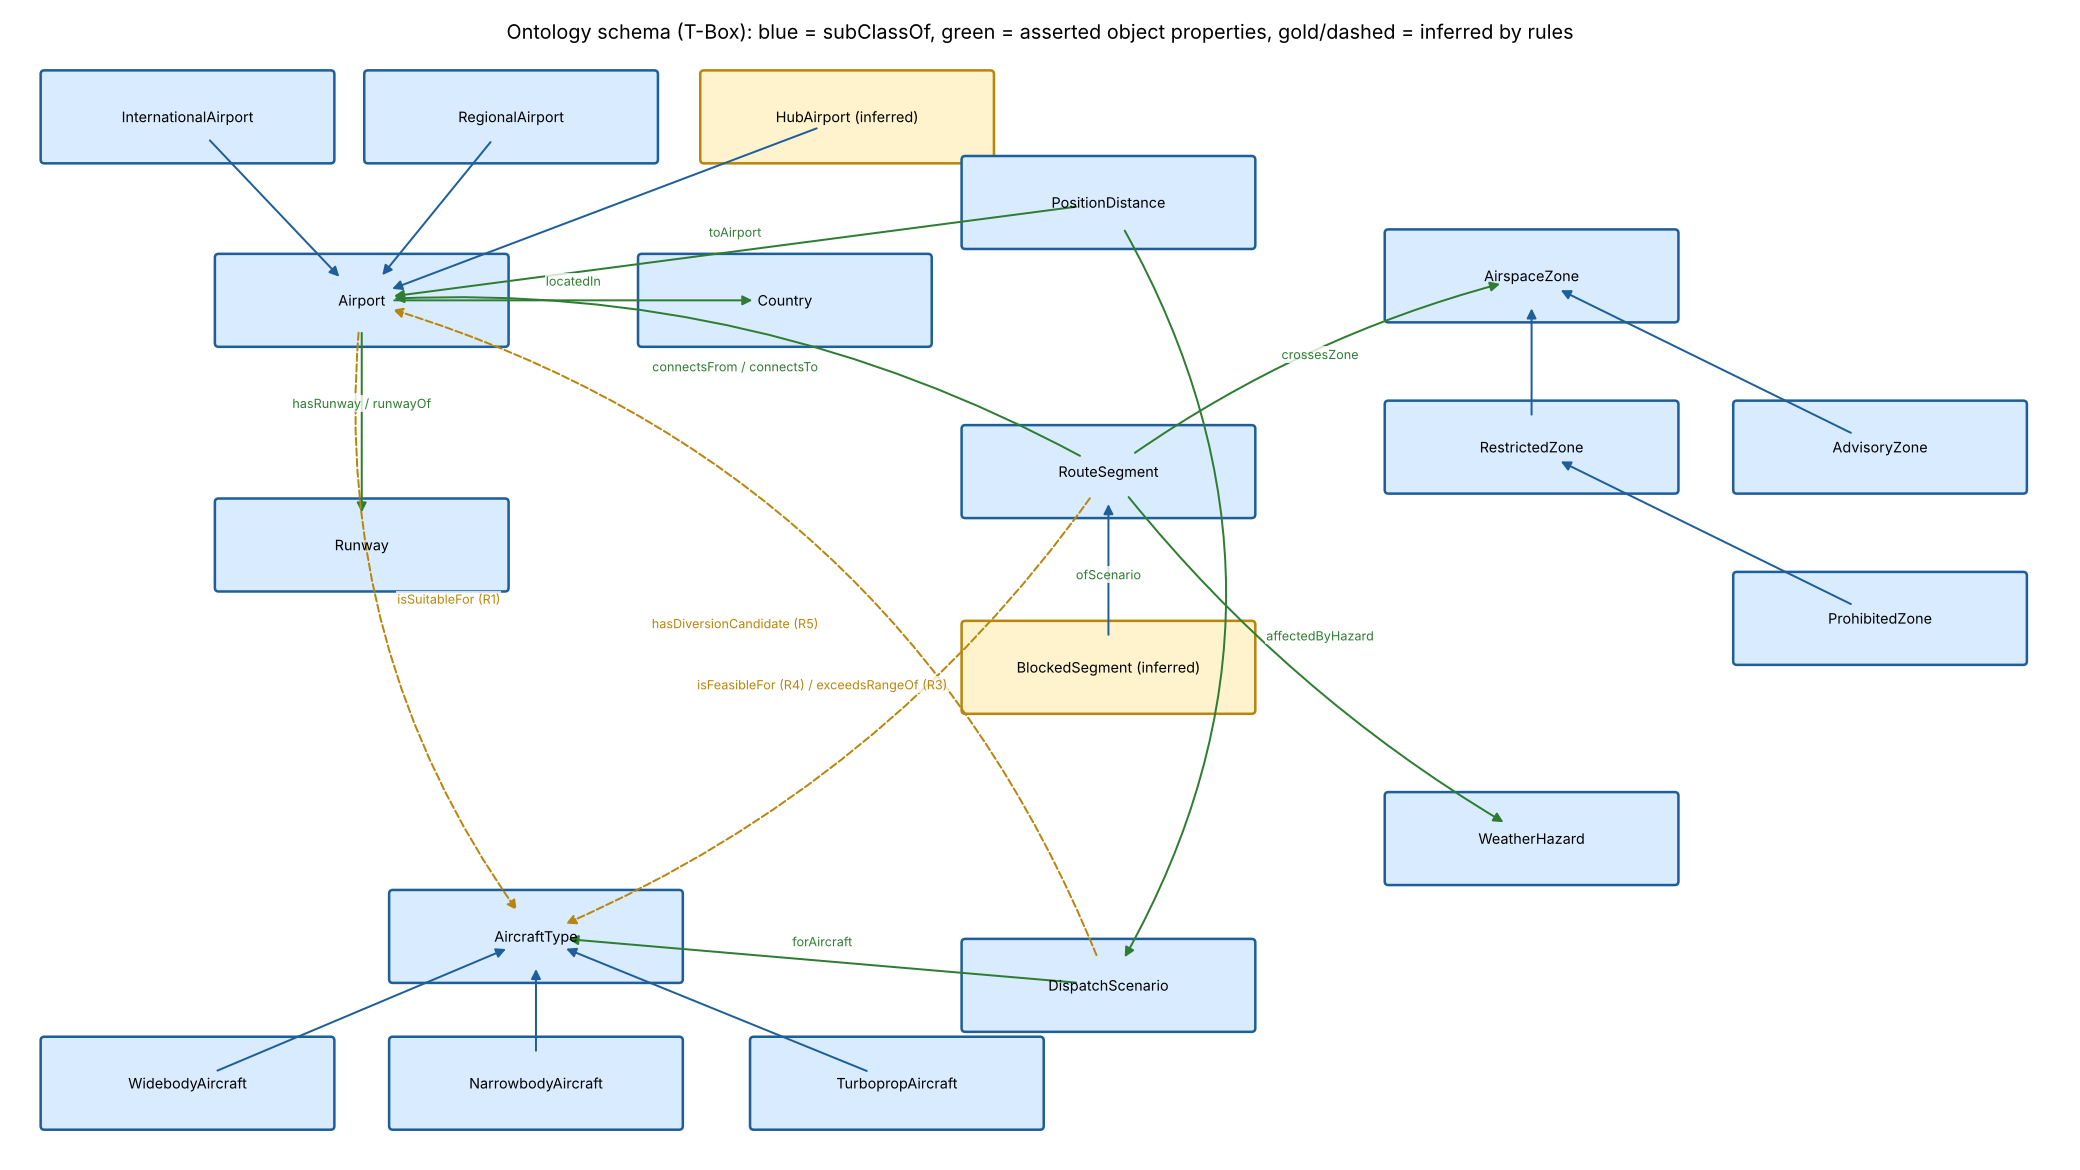
\includegraphics[width=0.88\textwidth]{ontology_schema.png}
\caption{SkyGraph Ontology Schema Diagram. Solid blue arrows represent \texttt{rdfs:subClassOf} inheritance hierarchies. Solid green arrows denote asserted object properties. Dashed gold arrows illustrate properties derived through inference rules.}
\label{fig:ontology_schema}
\end{figure*}

\subsection{Class Taxonomies}
Classes are structured into clean, mutually disjoint functional hierarchies:
\begin{itemize}
    \item \textbf{Aerodromes}: \texttt{fd:Airport} is specialized into \texttt{fd:InternationalAirport}, \texttt{fd:RegionalAirport}, and the inferred class \texttt{fd:HubAirport}.
    \item \textbf{Aircraft Categories}: \texttt{fd:AircraftType} subsumes \texttt{fd:WidebodyAircraft}, \texttt{fd:NarrowbodyAircraft}, and \texttt{fd:TurbopropAircraft}.
    \item \textbf{Route Infrastructure}: \texttt{fd:RouteSegment} represents an undirected airway link between two airports. The subclass \texttt{fd:BlockedSegment} is dynamically assigned to segments obstructed by active hazards.
    \item \textbf{Airspace Boundaries}: \texttt{fd:AirspaceZone} is specialized into \texttt{fd:RestrictedZone} and \texttt{fd:AdvisoryZone}. Furthermore, \texttt{fd:ProhibitedZone} is defined as a subclass of \texttt{fd:RestrictedZone}.
    \item \textbf{Environmental and Operational Context}: Classes include \texttt{fd:WeatherHazard}, \texttt{fd:Runway}, \texttt{fd:Country}, \texttt{fd:DispatchScenario}, and \texttt{fd:PositionDistance}.
\end{itemize}

\subsection{Formal Axioms and Schema Constraints}
To enforce data integrity, the T-Box incorporates several OWL constraint constructs:
\begin{itemize}
    \item \textbf{Disjointness Axioms}: \texttt{fd:Airport}, \texttt{fd:Runway}, \texttt{fd:AircraftType}, \texttt{fd:RouteSegment}, \texttt{fd:AirspaceZone}, and \texttt{fd:Country} are declared mutually disjoint via \texttt{owl:disjointWith}.
    \item \textbf{Cardinality and Existence}: Every \texttt{fd:Airport} must possess at least one runway (\texttt{owl:someValuesFrom fd:Runway}) and belong to exactly one country. Every \texttt{fd:RouteSegment} must have exactly one source and one destination airport.
    \item \textbf{Property Characteristics}: The property \texttt{fd:connectedTo} is declared symmetric. The property \texttt{fd:networkReachable} is declared both symmetric and transitive. The property \texttt{fd:hasRunway} has an explicit inverse \texttt{fd:runwayOf}.
    \item \textbf{Domain and Range Typing}: Explicit domains and ranges allow automatic type propagation. For example, the range of \texttt{fd:locatedIn} is \texttt{fd:Country}, which infers the country class for referenced geographic entities without manual typing.
\end{itemize}

Table~\ref{tab:tbox_constructs} summarizes the logical mechanisms applied across the ontology.

\begin{table}[htbp]
\caption{Logical Constructs Applied in the SkyGraph T-Box}
\label{tab:tbox_constructs}
\centering
\begin{tabular}{lp{5.2cm}}
\toprule
\textbf{Construct} & \textbf{Application and Functional Scope} \\
\midrule
\texttt{rdfs:subClassOf} & Specializes airports, aircraft classes, airspace zones, and blocked segments. \\
\texttt{rdfs:subPropertyOf} & Subsumes \texttt{connectsFrom} and \texttt{connectsTo} under \texttt{hasEndpoint}. \\
\texttt{owl:inverseOf} & Binds \texttt{hasRunway} and \texttt{runwayOf}. \\
\texttt{owl:SymmetricProperty} & Bidirectional connectivity for \texttt{connectedTo}. \\
\texttt{owl:TransitiveProperty} & Recursive network reachability for \texttt{networkReachable}. \\
\texttt{owl:disjointWith} & Prevents cross-type classification errors between all primary entities. \\
\texttt{owl:Restriction} & Enforces strict cardinality on runway presence and segment endpoints. \\
Rules R0 to R6 & Evaluates numerical thresholds not expressible in standard OWL 2 RL. \\
\bottomrule
\end{tabular}
\end{table}

\section{Knowledge Graph Construction and GraphDB}

\subsection{A-Box Population}
The knowledge graph instance file (\texttt{RDF\_Knowledge\_Graph/flight\_dispatch\_kg.ttl}) was synthesized directly from the cleaned tabular data. To demonstrate transparent inference, specific types were intentionally omitted from the explicit A-Box:
\begin{itemize}
    \item Country instances (such as \texttt{fdr:country-PK}) were asserted without \texttt{rdf:type fd:Country}. The class is inferred via the range axiom on \texttt{fd:locatedIn}.
    \item Aircraft individuals were asserted only under their specific subclass (e.g., \texttt{fd:WidebodyAircraft}), leaving the superclass \texttt{fd:AircraftType} to be derived through RDFS subclass inheritance.
\end{itemize}

\subsection{Graph Metrics}
The complete knowledge graph was validated against schema constraints. Table~\ref{tab:graph_metrics} details the structural metrics of the explicit and inferred graph.

\begin{table}[htbp]
\caption{Knowledge Graph Triple and Entity Metrics}
\label{tab:graph_metrics}
\centering
\begin{tabular}{lr}
\toprule
\textbf{Metric Description} & \textbf{Count} \\
\midrule
Explicit A-Box Triples (\texttt{flight\_dispatch\_kg.ttl}) & 2,105 \\
Explicit T-Box Triples (\texttt{flight\_dispatch\_ontology.ttl}) & 259 \\
Total Inferred Triples (\texttt{inferred\_facts.ttl}) & 3,048 \\
Modeled Aerodromes & 38 \\
Physical Runways & 60 \\
Route Network Segments & 153 \\
Inferred Blocked Segments & 45 \\
Inferred Hub Airports & 5 \\
Constraint Validation Violations & 0 \\
\bottomrule
\end{tabular}
\end{table}

\begin{figure*}[htbp]
\centering
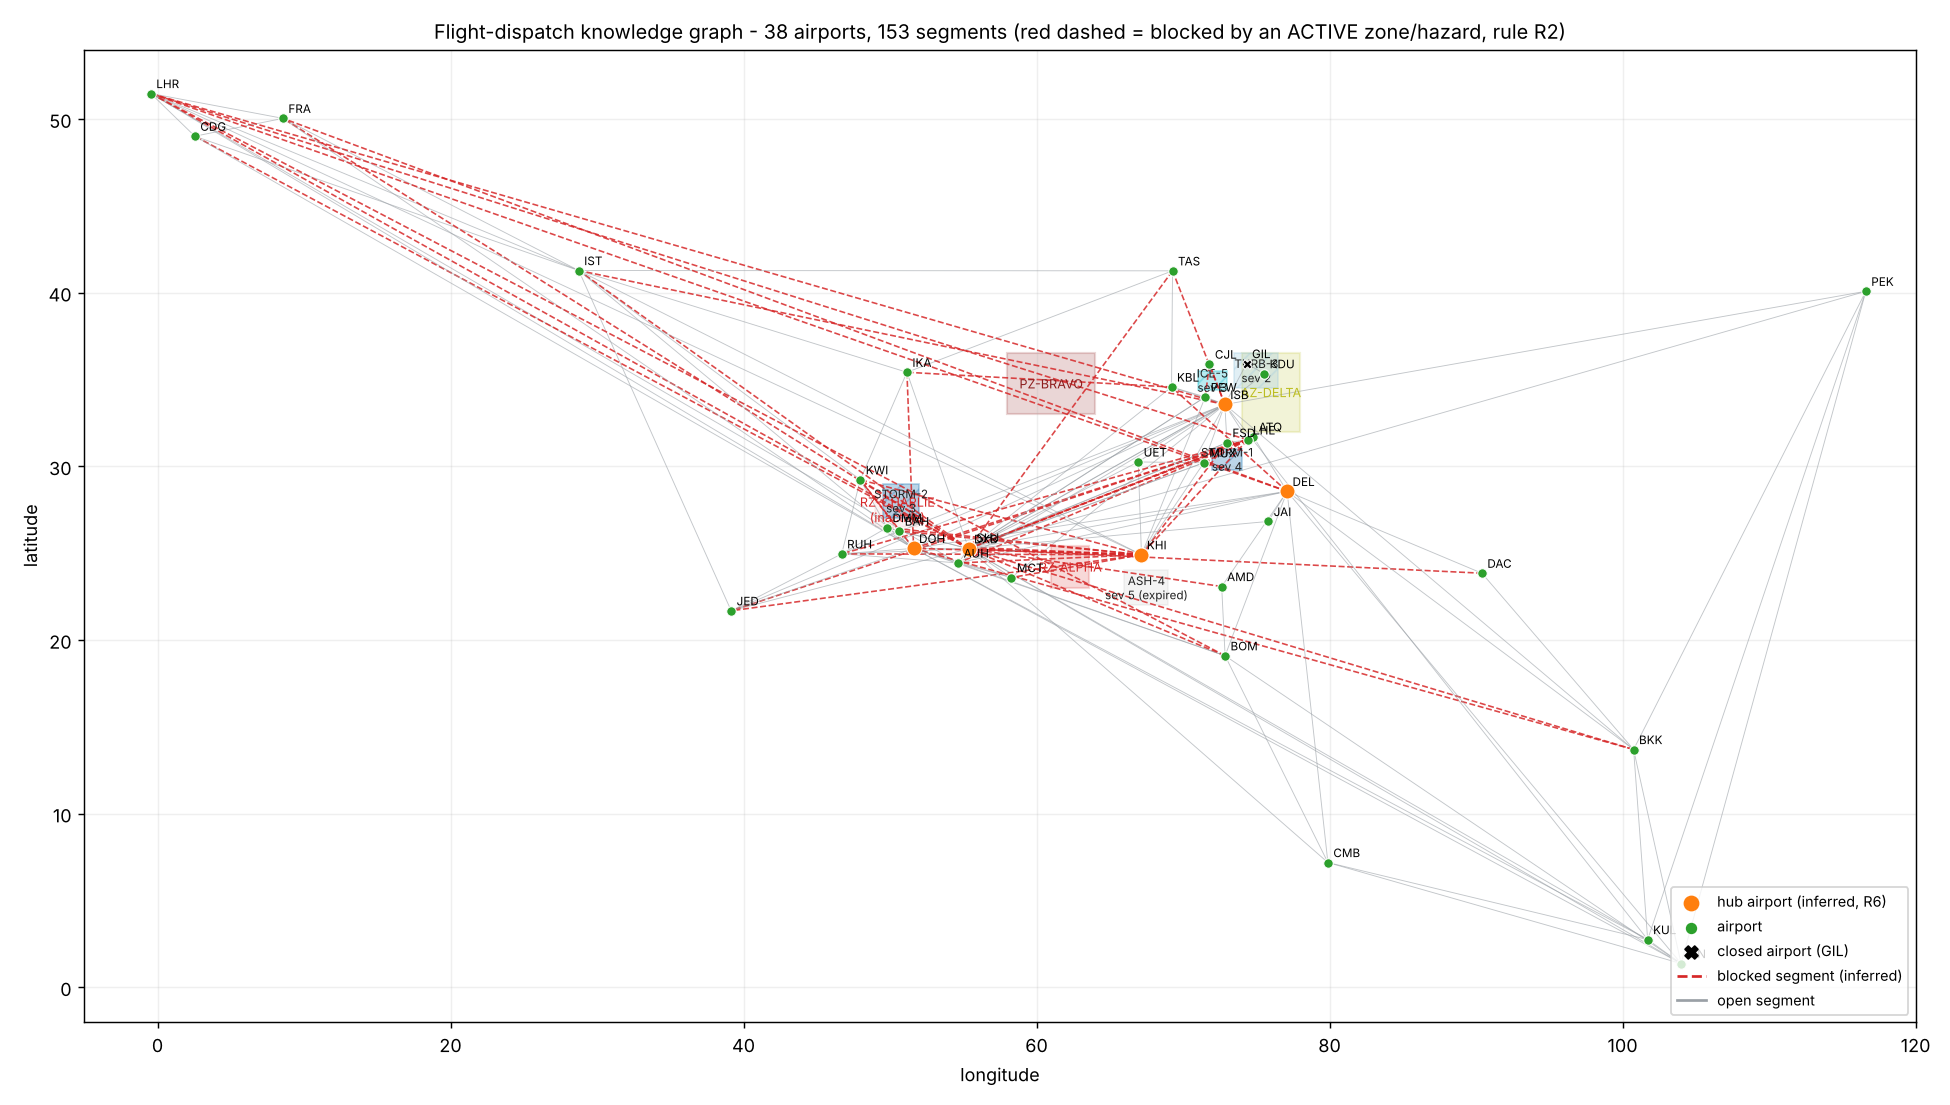
\includegraphics[width=0.88\textwidth]{kg_network_overview.png}
\caption{Complete Route Network Overview. Major hub airports are highlighted in orange. Inoperative airports are marked with red cross markers. Red dashed lines designate segments inferred as blocked by active restricted zones or severe weather hazards.}
\label{fig:network_overview}
\end{figure*}

\subsection{GraphDB Deployment Architecture}
The graph was verified for deployment in Ontotext GraphDB according to the procedure documented in \texttt{GRAPHDB\_GUIDE.md}:
\begin{enumerate}
    \item A dedicated repository was initialized using the standard \texttt{OWL2-RL (Optimized)} rule profile.
    \item The ontology file and the A-Box instance file were loaded via the GraphDB import workbench.
    \item Domain dispatch rules R0 through R6 were executed as a unified SPARQL Update sequence (\texttt{SPARQL\_Queries/rules/run\_all\_rules.ru}).
    \item Visual graph exploration was confirmed by expanding connections centered on Islamabad International Airport (\texttt{fdr:airport-OPIS}).
\end{enumerate}

Figure~\ref{fig:network_overview} visualizes the global topology of the network, highlighting inferred hubs, closed airports, and blocked route corridors.

\section{Rule-Based Symbolic Reasoning}

Standard OWL 2 RL description logics cannot express relational arithmetic comparisons, such as comparing a dynamic runway length against an aircraft threshold, or checking remaining flight range against geographic coordinates. We bridge this limitation using seven operational rules (R0 through R6). These rules are implemented both as portable SPARQL 1.1 Update scripts and in a deterministic Python forward-chaining reasoner (\texttt{src/reasoner.py}).

\subsection{Rule Formulations}

\textbf{Rule R0 (Longest Runway Aggregation):}
For each airport, determine the maximum length among all associated physical runways:
\begin{equation}
    L_{\max}(A) = \max \{ \text{length}(R) \mid \text{hasRunway}(A, R) \}
\end{equation}
This materializes the triple \texttt{(A, fd:longestRunwayM, }$L_{\max}$\texttt{)}.

\textbf{Rule R1 (Airport Suitability):}
An airport $A$ is suitable for aircraft $C$ if its longest runway meets or exceeds the aircraft's minimum required runway:
\begin{equation}
    L_{\max}(A) \ge \text{minRunway}(C) \implies \text{isSuitableFor}(A, C)
\end{equation}

\textbf{Rule R2 (Airspace and Hazard Blocking):}
A route segment $S$ is blocked if it crosses an active restricted zone, or an active weather hazard with a severity index of 3 or greater:
\begin{align}
    \text{crossesZone}(S, Z) \land \text{RestrictedZone}(Z) \land \text{isActive}(Z) &\implies \text{blockedBy}(S, Z) \\
    \text{affectedBy}(S, H) \land \text{severity}(H) \ge 3 \land \text{isActive}(H) &\implies \text{blockedBy}(S, H)
\end{align}
Any segment with at least one \texttt{blockedBy} relation is dynamically asserted as an instance of \texttt{fd:BlockedSegment}.

\textbf{Rule R3 (Range Exceedance):}
A route segment $S$ exceeds the operational limit of aircraft $C$ if the segment distance is greater than the aircraft maximum range:
\begin{equation}
    \text{distance}(S) > \text{range}(C) \implies \text{exceedsRangeOf}(S, C)
\end{equation}

\textbf{Rule R4 (Segment Feasibility):}
A segment $S$ connecting airports $A_1$ and $A_2$ is feasible for aircraft $C$ if and only if the segment is not blocked, does not exceed aircraft range, and both endpoints are operational and suitable:
\begin{align}
    \neg \text{BlockedSegment}(S) &\land \neg \text{exceedsRangeOf}(S, C) \nonumber \\
    &\land \text{isSuitableFor}(A_1, C) \land \text{isOperational}(A_1) \nonumber \\
    &\land \text{isSuitableFor}(A_2, C) \land \text{isOperational}(A_2) \nonumber \\
    &\implies \text{isFeasibleFor}(S, C)
\end{align}

\textbf{Rule R5 (Emergency Diversion Selection):}
For an in-flight dispatch scenario $Sc$ with remaining range $D_{\text{rem}}$, airport $A$ is a valid diversion candidate if it is operational, suitable for the aircraft, and within the remaining range distance:
\begin{align}
    \text{distance}(Sc, A) \le D_{\text{rem}} &\land \text{isSuitableFor}(A, C) \land \text{isOperational}(A) \nonumber \\
    &\implies \text{hasDiversionCandidate}(Sc, A)
\end{align}

\textbf{Rule R6 (Hub Aerodrome Classification):}
An airport $A$ is classified as a hub if the count of its incident route segments is 14 or greater:
\begin{equation}
    \text{degree}(A) \ge 14 \implies \text{rdf:type}(A, \text{fd:HubAirport})
\end{equation}

\subsection{Demonstrated Inference Traces}

The reasoning engine demonstrates seven transparent inference chains:
\begin{enumerate}
    \item \textbf{Airport Suitability (R0 + R1)}: Islamabad International Airport (\texttt{OPIS}) has runway 15/33 measuring 3,658 m. The Airbus A380-800 requires 3,000 m. R0 derives \texttt{fd:longestRunwayM 3658}, which satisfies R1, deriving \texttt{fdr:airport-OPIS fd:isSuitableFor fdr:aircraft-A380-800}. Conversely, Skardu Airport (\texttt{OPSD}) has a 2,743 m runway. Because $2743 < 3000$, suitability for the A380 is rejected.
    \item \textbf{Restricted Airspace Blocking (R2)}: Segment Karachi to Dubai (\texttt{fdr:segment-OPKC-OMDB}) intersects Restricted Zone Alpha (\texttt{fdr:zone-RZ-ALPHA}). Because the zone is active, R2 derives \texttt{fd:blockedBy} and assigns \texttt{rdf:type fd:BlockedSegment}.
    \item \textbf{Subclass Axiom Propagation (RDFS + R2)}: Prohibited Zone Bravo (\texttt{fdr:zone-PZ-BRAVO}) is asserted only as a \texttt{fd:ProhibitedZone}. The ontology defines \texttt{fd:ProhibitedZone rdfs:subClassOf fd:RestrictedZone}. The engine infers that the zone is a restricted area. Consequently, the Islamabad to London segment (\texttt{fdr:segment-OPIS-EGLL}) crossing it is derived as blocked.
    \item \textbf{Emergency Diversion Identification (R5)}: Scenario S1 models an A380 with 1,500 km remaining fuel. Jinnah International Airport in Karachi (\texttt{OPKC}) is 318.8 km away, fully operational, and possesses a 3,400 m runway. Rule R5 derives \texttt{fdr:scenario-S1 fd:hasDiversionCandidate fdr:airport-OPKC}.
    \item \textbf{Range Exceedance (R3)}: The direct segment Islamabad to Dubai measures 1,925.5 km. The ATR 72-600 has a maximum range of 1,528 km. R3 derives \texttt{fdr:segment-OPIS-OMDB fd:exceedsRangeOf fdr:aircraft-ATR72-600}.
    \item \textbf{Hub Classification (R6)}: Dubai International Airport (\texttt{OMDB}) connects to 34 route segments. Because $34 \ge 14$, R6 classifies it as \texttt{fd:HubAirport}. Nationwide and regional hubs inferred include DEL, DOH, DXB, ISB, and KHI.
    \item \textbf{OWL Structural Axioms}: Bidirectional connectivity is inferred across all 153 segments from the symmetric declaration on \texttt{fd:connectedTo}. The inverse axiom derives \texttt{fd:runwayOf} for all 60 runways.
\end{enumerate}

\subsection{Negative Verification Checks}
To guarantee that inference rules do not over-generalize, the test suite verifies negative conditions:
\begin{itemize}
    \item \textbf{Inactive Airspace}: Restricted Zone Charlie (\texttt{RZ-CHARLIE}) is inactive. Although 17 flight segments cross its boundary, none are derived as blocked.
    \item \textbf{Advisory Airspace}: Advisory Zone Delta (\texttt{AZ-DELTA}) intersects 7 flight segments. Because advisory areas never block traffic, no segment is blocked.
    \item \textbf{Minor Weather Hazards}: Weather Hazard \texttt{TURB-3} has severity 2. Because $2 < 3$, it does not trigger segment blockage.
    \item \textbf{Expired Hazards}: Hazard \texttt{ASH-4} has an active flag set to false. All 3 intersecting segments remain open.
    \item \textbf{Closed Airfields}: Gilgit Airport (\texttt{OPGT}) has \texttt{fd:isOperational false}. All incident segments are rejected from the feasible subgraph.
\end{itemize}

\section{SPARQL Query Suite and Empirical Results}

A suite of 16 SPARQL queries was developed and executed to validate the graph against the competency questions. Table~\ref{tab:sparql_suite} lists each query file, the primary semantic feature tested, and the expected result count.

\begin{table}[htbp]
\caption{SPARQL Query Validation Suite}
\label{tab:sparql_suite}
\centering
\begin{tabular}{lllc}
\toprule
\textbf{File} & \textbf{Semantic Feature Demonstrated} & \textbf{Rows} \\
\midrule
\texttt{q01} & Basic graph pattern matching & 10 \\
\texttt{q02} & Numeric constraint filtering with \texttt{FILTER} & 37 \\
\texttt{q03} & Conditional join using \texttt{OPTIONAL} and \texttt{FILTER} & 32 \\
\texttt{q04} & Bidirectional union via \texttt{UNION} & 23 \\
\texttt{q05} & Aggregation grouping with \texttt{COUNT} and \texttt{GROUP BY} & 21 \\
\texttt{q06} & Inferred blockage aggregation (Rule R2) & 5 \\
\texttt{q07} & Multi-hop traversal across four entity classes & 14 \\
\texttt{q08} & Arbitrary-depth reachability via property paths & 37 \\
\texttt{q09} & Two-leg route search over inferred feasible graph (R4) & 30 \\
\texttt{q10} & Emergency diversion ranking by distance (Rule R5) & 18 \\
\texttt{q11} & Negation using \texttt{FILTER NOT EXISTS} & 2 \\
\texttt{q12} & Aircraft suitability aggregation (Rules R0, R1) & 6 \\
\texttt{q13} & Boolean feasibility verification using \texttt{ASK} & 1 \\
\texttt{q14} & Transparent causal explanation using \texttt{BIND} & 1 \\
\texttt{q15} & Two-hop sequence paths over suitable airports & 32 \\
\texttt{q16} & Inferred hub aerodrome identification (Rule R6) & 5 \\
\bottomrule
\end{tabular}
\end{table}

\subsection{Selected Query Demonstrations}

\textbf{Emergency Diversion Candidates (Query \texttt{q10}):}
Listing \ref{lst:q10} displays the SPARQL implementation for CQ10. It identifies valid diversion airfields for Scenario S1, ordered by proximity.

\begin{lstlisting}[language=SPARQL, caption={Query q10: Diversion Candidates for Scenario S1}, label={lst:q10}]
PREFIX fd:  <https://krr.example.org/fd/ontology#>
PREFIX fdr: <https://krr.example.org/fd/data/>

SELECT ?iata ?name ?distance WHERE {
  fdr:scenario-S1 fd:hasDiversionCandidate ?a .
  ?a fd:iataCode ?iata ;
     rdfs:label ?name .
  ?pd fd:ofScenario fdr:scenario-S1 ;
      fd:toAirport ?a ;
      fd:distanceKm ?distance .
}
ORDER BY ?distance
\end{lstlisting}

Table~\ref{tab:q10_results} displays the top diversion candidates returned by query \texttt{q10}.

\begin{table}[htbp]
\caption{Diversion Candidates for Scenario S1 (Query q10)}
\label{tab:q10_results}
\centering
\begin{tabular}{llr}
\toprule
\textbf{IATA Code} & \textbf{Aerodrome Name} & \textbf{Distance (km)} \\
\midrule
KHI & Jinnah International Airport & 318.8 \\
MCT & Muscat International Airport & 599.9 \\
UET & Quetta International Airport & 651.6 \\
SHJ & Sharjah International Airport & 854.4 \\
DXB & Dubai International Airport & 869.7 \\
AMD & Sardar Vallabhbhai Patel Airport & 902.4 \\
\bottomrule
\end{tabular}
\end{table}

\textbf{Blocked Segments by Primary Cause (Query \texttt{q06}):}
Query \texttt{q06} inspects segments obstructed by active environmental hazards and restricted zones. Table~\ref{tab:q06_results} presents the breakdown of blocked segments across all causes.

\begin{table}[htbp]
\caption{Blocked Flight Segments Grouped by Cause (Query q06)}
\label{tab:q06_results}
\centering
\begin{tabular}{llr}
\toprule
\textbf{Cause Entity} & \textbf{Hazard Description} & \textbf{Blocked Segments} \\
\midrule
\texttt{fdr:zone-RZ-ALPHA} & Restricted Zone Alpha (Naval) & 15 \\
\texttt{fdr:hazard-STORM-1} & Thunderstorm Cell Punjab & 13 \\
\texttt{fdr:hazard-STORM-2} & Thunderstorm Line Northern Gulf & 10 \\
\texttt{fdr:zone-PZ-BRAVO} & Prohibited Zone Bravo & 7 \\
\texttt{fdr:hazard-ICE-5} & Icing Band Hindu Kush & 3 \\
\bottomrule
\end{tabular}
\end{table}

\section{Constraint-Aware Routing Evaluation}

To validate that symbolic inference directly supports path planning, the router (\texttt{src/routing.py}) executes Dijkstra's algorithm over the graph formed by edges satisfying \texttt{fd:isFeasibleFor}.

\begin{figure}[htbp]
\centering
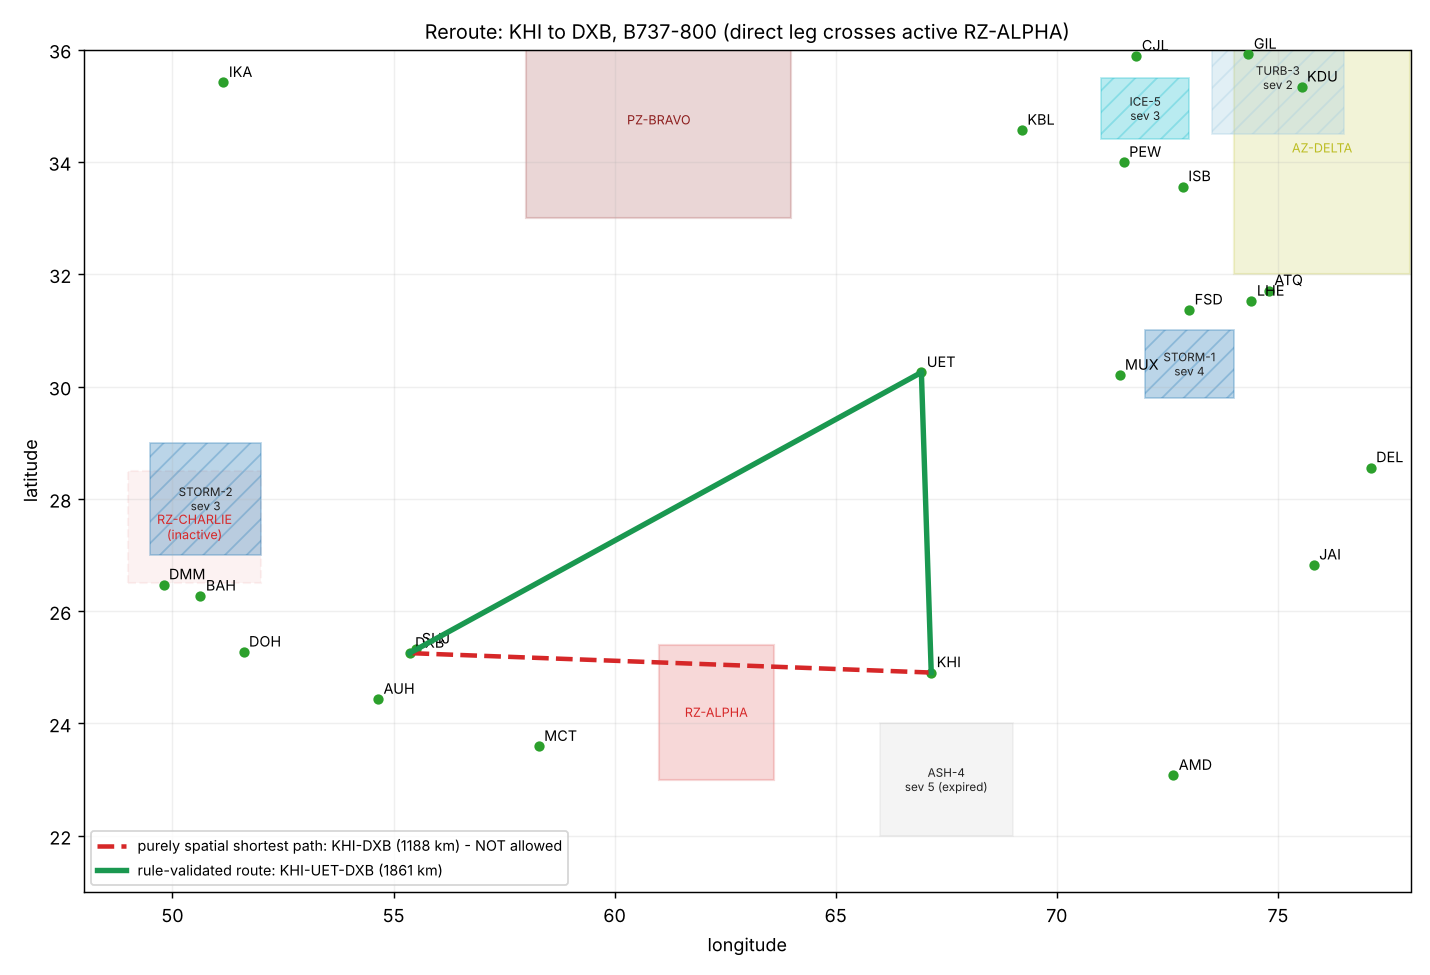
\includegraphics[width=0.48\textwidth]{reroute_khi_dxb.png}
\caption{Reroute planning between Karachi (KHI) and Dubai (DXB). The direct path of 1,188 km is blocked by active Restricted Zone Alpha. The rule-guided engine routes the Boeing 737-800 via Quetta (UET) across two feasible legs totaling 1,861 km.}
\label{fig:reroute_khi_dxb}
\end{figure}

\begin{figure}[htbp]
\centering
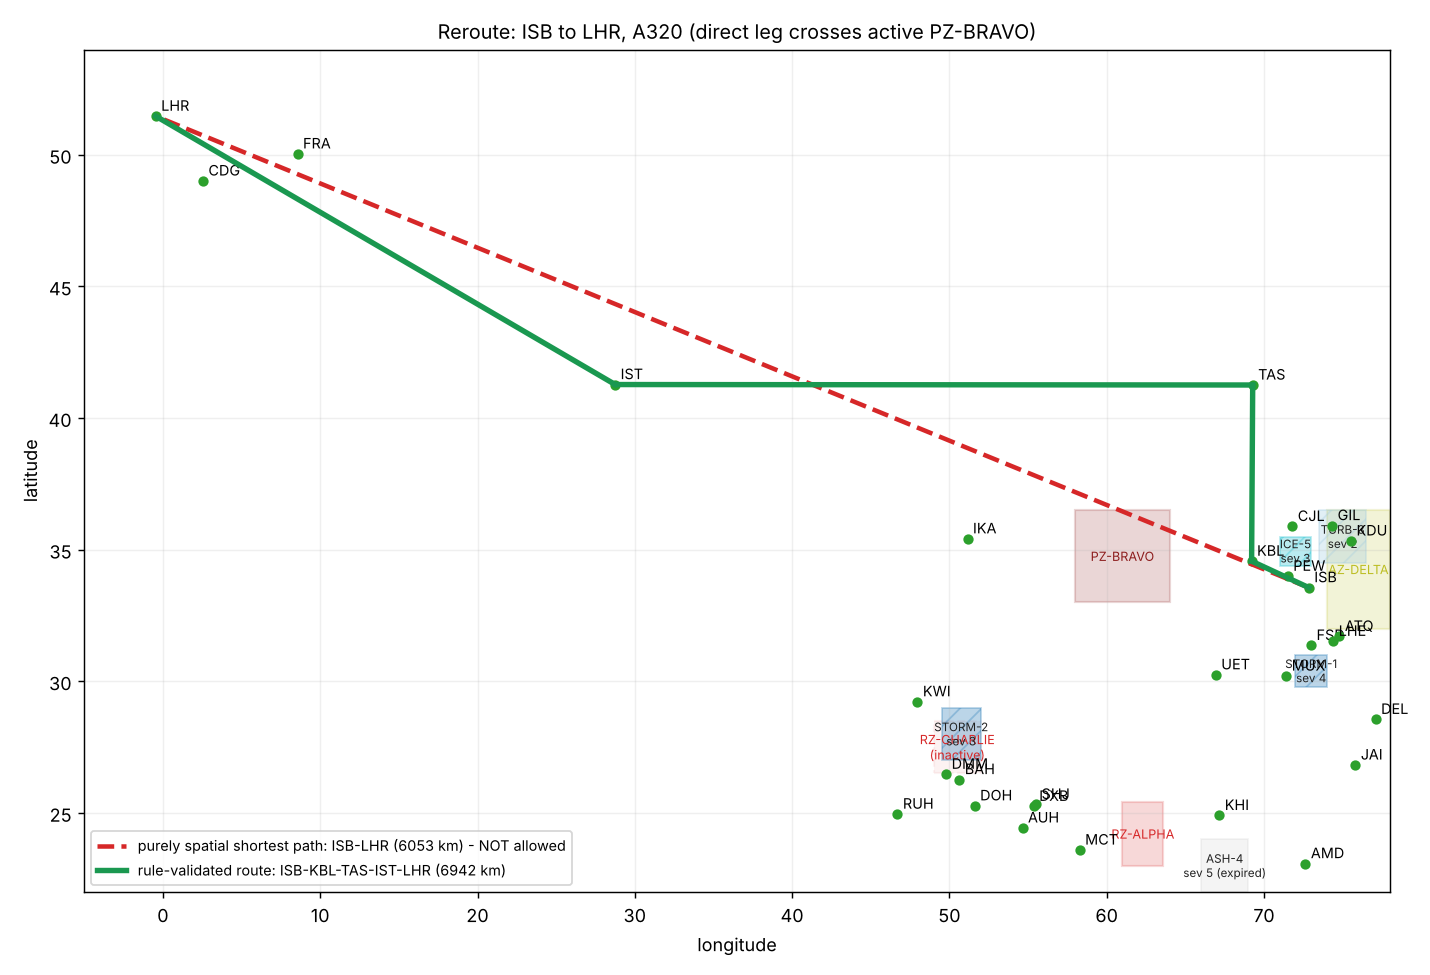
\includegraphics[width=0.48\textwidth]{reroute_isb_lhr.png}
\caption{Reroute planning between Islamabad (ISB) and London Heathrow (LHR) for an Airbus A320-200. Direct flight violates aircraft fuel range and crosses Prohibited Zone Bravo. The engine derives a 4-leg feasible route: ISB $\rightarrow$ KBL $\rightarrow$ TAS $\rightarrow$ IST $\rightarrow$ LHR.}
\label{fig:reroute_isb_lhr}
\end{figure}

Figure~\ref{fig:reroute_khi_dxb} illustrates a flight dispatch query from Karachi to Dubai for a Boeing 737-800. A standard spatial planner selects the direct segment of 1,188 km. SkyGraph identifies that the direct segment crosses Restricted Zone Alpha, rendering it infeasible via Rule R2. The engine computes the shortest constraint-valid alternative via Quetta (\texttt{KHI-UET-DXB}), covering 1,861.0 km across two verified legs.

Figure~\ref{fig:reroute_isb_lhr} shows a long-range routing challenge from Islamabad to London for an Airbus A320-200. The direct segment violates aircraft range (6,053 km versus 6,112 km maximum range with reserves) and intersects Prohibited Zone Bravo. SkyGraph synthesizes a multi-leg path through Kabul, Tashkent, and Istanbul (\texttt{ISB-KBL-TAS-IST-LHR}), totaling 6,941.7 km. Each individual leg is verified for airport runway compatibility, aircraft range limits, and operational airspace clearance.

\section{Work Progress and Contributions}

\subsection{Milestone Evaluation}
Iteration 1 requirements specified in the project work file have been completed in full. Table~\ref{tab:progress_status} outlines the delivery status across all functional areas.

\begin{table}[htbp]
\caption{Project Milestone and Delivery Status}
\label{tab:progress_status}
\centering
\begin{tabular}{lp{4.8cm}}
\toprule
\textbf{Functional Module} & \textbf{Delivery Status and Verification} \\
\midrule
Curated Aviation Dataset & Complete; 8 relational CSV tables cleaned and cross-referenced. \\
Competency Questions & Complete; 15 formal CQs mapped to graph queries. \\
OWL 2 RL Ontology & Complete; 19 classes, 38 properties, 8 reasoning constructs. \\
RDF Knowledge Graph & Complete; 2,105 explicit triples, 3,048 inferred facts. \\
Symbolic Reasoning & Complete; Rules R0 to R6 verified against baseline recomputation. \\
SPARQL Query Suite & Complete; 16 executable query files tested. \\
Automated Test Harness & Complete; 27 passing test cases (\texttt{src/tests.py}). \\
Interactive Demonstration & Ready; GraphDB guide and Protege verification documented. \\
\bottomrule
\end{tabular}
\end{table}

\subsection{Individual Contributions}
All team members contributed actively to the research, modeling, implementation, and documentation. Table~\ref{tab:member_contributions} outlines the specific division of responsibilities.

\begin{table}[htbp]
\caption{Team Member Technical Contributions}
\label{tab:member_contributions}
\centering
\begin{tabular}{lp{5.0cm}}
\toprule
\textbf{Member Name and ID} & \textbf{Primary Technical Responsibilities} \\
\midrule
Huzaifa Mudassar \newline (24i-0050) & \textbf{Domain Modeling and Ontology Design (T-Box)}: Conceptualized the aviation domain ontology in Protégé, established class taxonomies, defined object and datatype properties, specified domain/range restrictions, and formulated schema disjointness axioms. \\
\midrule
Abdul Samad \newline (24i-0095) & \textbf{Dataset Curation, ETL, and RDF Graph (A-Box)}: Curated aerodrome, runway, and aircraft datasets, implemented spatial precomputations for haversine distances and polygon intersection geometry, engineered the URI scheme, generated 2,105 RDF triples, and managed GraphDB repository deployment. \\
\midrule
Shaheed Khan \newline (24i-0037) & \textbf{SPARQL Queries and Symbolic Reasoning Engine}: Authored the 15 competency questions and the CQ-to-KG mapping table, implemented the 16 SPARQL queries, formulated the SPARQL Update inference rules (R0 to R6), and validated inferred facts against baseline recomputations. \\
\bottomrule
\end{tabular}
\end{table}

\section{Conclusion}
Iteration 1 of the SkyGraph project demonstrates the value of integrating symbolic knowledge representation into flight dispatch workflows. By combining an expressive OWL 2 RL ontology with forward-chaining production rules, the system eliminates infeasible flight paths prior to route optimization. The resulting flight plans are verifiable, operationally realistic, and fully explainable. The knowledge graph contains 2,105 explicit assertions and 3,048 derived inferences, successfully answering all 15 competency questions across 16 formal SPARQL queries. The system provides a solid, extensible foundation for subsequent phases involving neuro-symbolic link prediction and retrieval-augmented language interaction.

\begin{thebibliography}{00}
\bibitem{w3c_owl2} W3C OWL Working Group, ``OWL 2 Web Ontology Language Document Overview (Second Edition),'' W3C Recommendation, Dec. 2012. \url{https://www.w3.org/TR/owl2-overview/}
\bibitem{w3c_sparql} W3C SPARQL Working Group, ``SPARQL 1.1 Query Language,'' W3C Recommendation, Mar. 2013. \url{https://www.w3.org/TR/sparql11-query/}
\bibitem{icao_annex15} International Civil Aviation Organization, ``Aeronautical Information Services,'' ICAO Annex 15, 16th ed., Montreal, Canada, 2018.
\bibitem{openap} J. Sun, J. M. Hoekstra, and J. Ellerbroek, ``OpenAP: An Open-Source Aircraft Performance Model for Air Transport Studies and Flight Simulations,'' \textit{Aerospace}, vol. 7, no. 8, p. 104, 2020.
\bibitem{ourairports} OurAirports Open Data Initiative, ``Global Aerodrome and Runway Database,'' 2024. \url{https://ourairports.com/data/}
\bibitem{eurocontrol_swim} EUROCONTROL, ``System-Wide Information Management (SWIM) Concept and Architecture,'' European Organisation for the Safety of Air Navigation, Brussels, Belgium, Tech. Rep., 2021.
\end{thebibliography}

\end{document}
